\section{提案手法}
\label{chap:proposed_method}
\subsection{提案手法の概要}
\label{sec:proposed_method_overviews}
本研究ではスピーカから出た音が対象平面に反射してマイクにて検出された音を使用し、発する音の周波数と反射音の強度の関係を使うことによって、対象平面の方位角方向を推定する手法を提案する。この提案手法の概要について、\figref{proposed_method_overview}にて示す。

推定手法としては、二通りの方法によって、対象面の方位角方向とマイクで取得した音の関係をモデル化を行った。\\
一つ目は音響、物理の音の反射モデルを参考にすることで、方位角度と反射音の関係をモデル化を行った。詳細は\secref{self_by_myself}で示す。\\
二つ目は無響室、実環境二つの環境で集めたデータに対して、サポートベクター回帰を用いて、モデル化を行った詳細は\secref{svr_method}で示す。

\begin{figure}[ht]
    \centering
    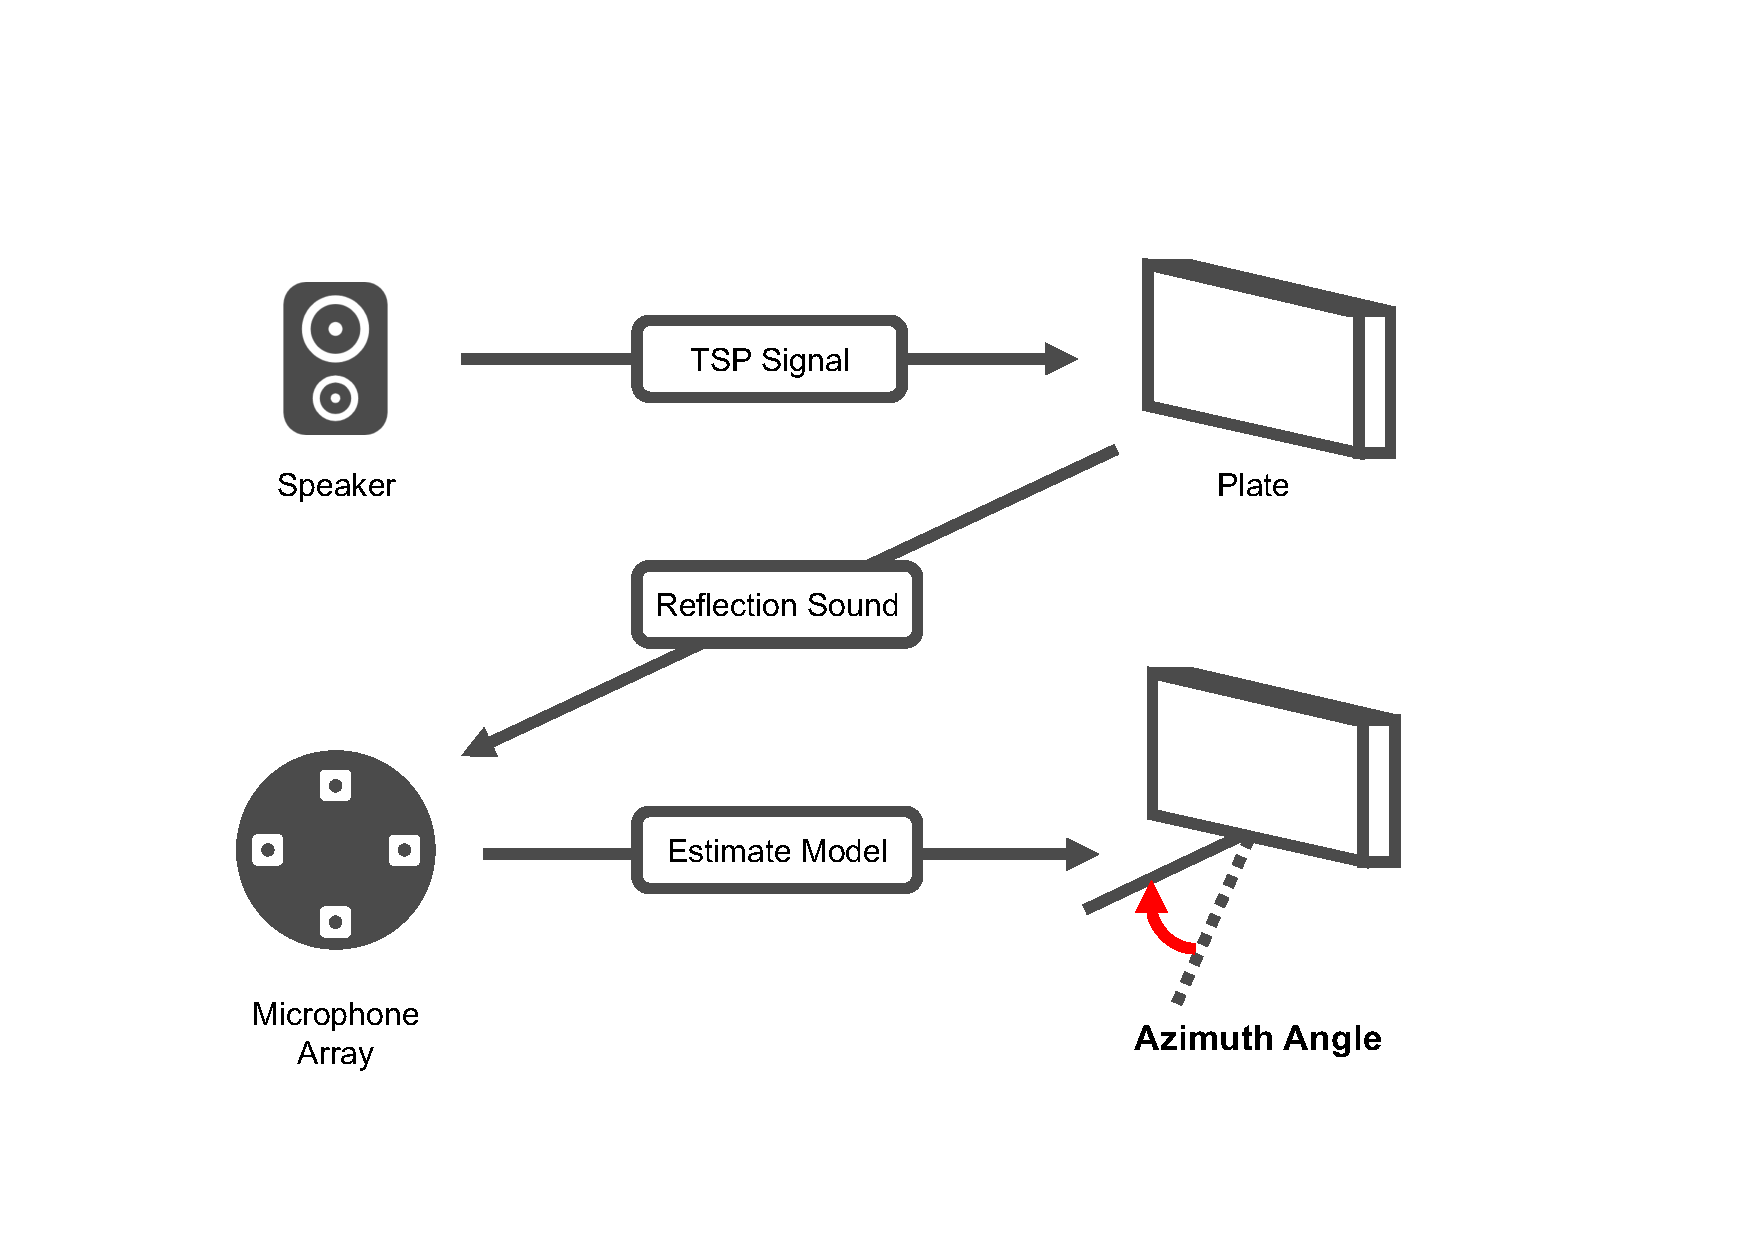
\includegraphics[width=\linewidth]{images/2_proposed_method.pdf}
    \caption{The overview of the proposed method}
    \label{fig:proposed_method_overview}
\end{figure}

\subsection{方位角推定モデルの作成}
\label{sec:self_by_myself}
\subsubsection{音波の反射特性}
光の可視範囲の波長が780[nm] $\sim$ 380[nm]なのに対して、音の可聴範囲での波長は17[m] (20[Hz]) $\sim$ 17[mm] (20[kHz])で長さの差が1000倍もある。そのため、光に比べて、音波はその周波数によって反射特性に変化がでる\cite{fujiwara1997diffusereflection}。

周波数の違いによる反射特性の変化を\tabref{reflection_chara}に示す。
音波の反射はlow(低域)では、小さな傾きや凹凸には関係なく鏡面反射する。Middle(中域)では、物理の反射の法則に乗っ取り鏡面反射する。最後に、High(高域)では、拡散反射する。
本論文では、中域から高域に渡って、反射特性が変化することに着目する。
低域を無視した理由としては、低域では、マイクとスピーカの入力音圧レベルと出力音圧レベルの周波数特性が著しく小さくなることが多いという点と低域は生活雑音が多い点の2点の問題が挙げられる。
それぞれの反射のエネルギーに着目すると、鏡面反射では,反射音は入射角に応じて,ある定まった方向にのみ反射する.それに対し,拡散反射では,入射角により反射する音のエネルギーは影響されるものの,すべての方向に一様に反射する.

\figref{specular_strong}のように、鏡面反射した音がマイクに入りやすい面の角度の場合、中域では鏡面反射した音波を主に観測し,高域では拡散反射した音波を観測する。鏡面反射で観測されるエネルギーの方が大きいため,周波数の変化により全体として観測されるエネルギーが減少していくと考えられる.

\figref{specular_weak}のように、鏡面反射した音がマイクに入りにくい面の角度の場合、中域では鏡面反射した音波を観測することは難しく,高域で拡散反射した音波が増えるに従い観測される音波のエネルギーも増加していくと考えられる.

このように、中域(鏡面反射)・高域(拡散反射)のエネルギーの差と物体面の方位角にはある関係があると考えられる。

\begin{table}[t]
  \setcounter{table}{0}
  \begin{center}
  \caption{Response of reflection in various frequencies.}
  \vspace{1zh}
  \label{tab:reflection_chara}
  \begin{tabular}{c|c|c}\hline
        & Frequency & Characteristic\\\hline
        Low & 20[Hz]-100[Hz] &
        \begin{tabular}{c}
            Perfect specular
        \end{tabular}\\\hline
        Middle & 100[Hz]-1[kHz] & Specular\\\hline
        High & 1[kHz]-20[kHz] & Diffuse\\\hline
  \end{tabular}
  \end{center}
\end{table}

\begin{figure}[t]
    \centering
    \subfigure[Case that specularly reflected sound enters the microphone]{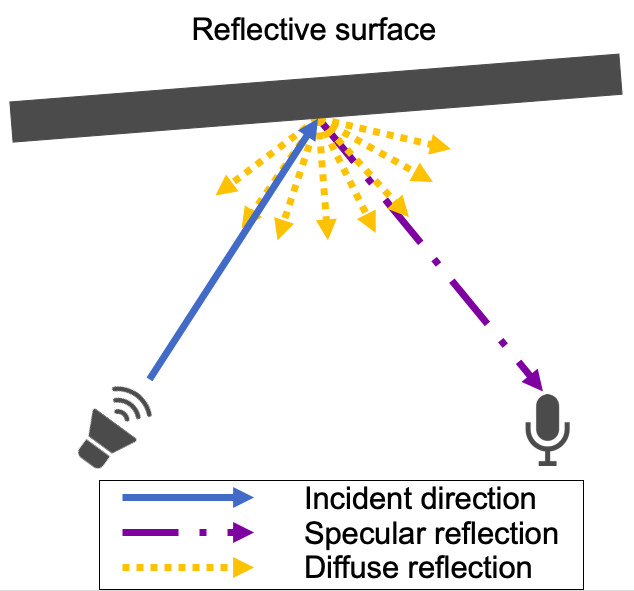
\includegraphics[width=0.45\linewidth]{images/2_specular_strong.png}\label{fig:specular_strong}}
    \subfigure[Case that diffusely reflected sound enters the microphone]{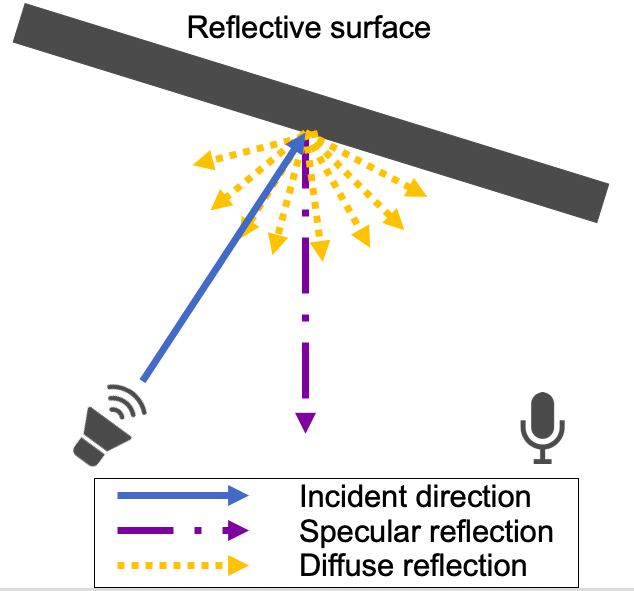
\includegraphics[width=0.45\linewidth]{images/2_specular_weak.png}\label{fig:specular_weak}}
    \caption{The energy acquired by the microphone changes as the frequency of the sound and the angle of the surface's azimuth change.}
    \label{fig:freq&normal}
\end{figure}

\clearpage

\subsubsection{反射音のモデル化}
\label{sec:light_model}
光学における物体面での反射モデルを参考にすると, 反射音は鏡面反射と拡散反射の和でマイクに入ってくると考える。光と違い、音は周波数に応じて,鏡面反射, 拡散反射の割合が変化していくものと考えられる.

\begin{figure}[t]
  \begin{center}
  \vspace{1zh}
    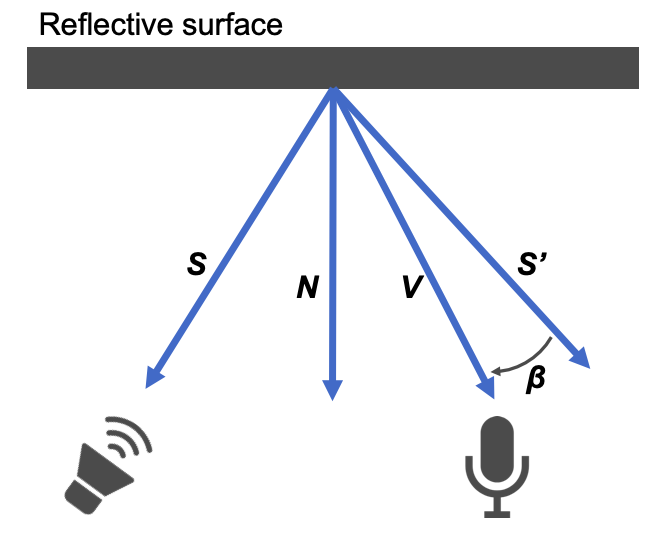
\includegraphics[width=0.7\linewidth]{images/2_model_base_environment.png}   
  \end{center}
  \caption{Model environment}
  \label{fig:model_env}
\end{figure}

\figref{model_env}のような環境において、レイトレーシングにより、仮想的な音波の線を用いて反射について考える。音源が$\mathbf{S}$から入射した際に平面上のある点$Q$点での反射したとする。ここで、面の方向を$\mathbf{N}$, 音波が鏡面反射した際の反射方向を$\mathbf{S'}$, 観測する方向を$\mathbf{V}$とした時、$\mathbf{S'}$と$\mathbf{V}$の角度の差を$\beta$とおく。
ある点$Q$で反射してマイクで取得できる音のエネルギー$E$は以下の用に表す事ができる。
\begin{equation}
\begin{aligned}
    \label{equ:all-reflection}
        E(f, \mathbf{S}, \mathbf{N}, \mathbf{V}) 
        = \gamma_\mathrm{spe}(f) e_\mathrm{spe}(\mathbf{S}, \mathbf{N}, \mathbf{V})\\
        + \gamma_\mathrm{dif}(f) e_\mathrm{dif}(\mathbf{S}, \mathbf{N}).
\end{aligned}
\end{equation}

ただし,$ e_\mathrm{spe}, e_\mathrm{dif} $は,ある基準の音源における,マイクが受け取る鏡面反射,拡散反射音のエネルギー,$\gamma_\mathrm{spe}, \gamma_\mathrm{dif} $は, ある基準の音源における,鏡面反射率、拡散反射率のをそれぞれ示す.また、$ e_\mathrm{spe}, e_\mathrm{dif} $について詳細はそれぞれ以下にて説明している。

このとき、今回反射以外でのエネルギー損失をないと仮定し、$\gamma_\mathrm{spe} + \gamma_\mathrm{dif} = 1 $と考える。反射音における拡散反射率の関数$\gamma_\mathrm{dif}$は佐久間らが実測によって求めた周波数が変化した際の拡散反射率の変化の結果から引用した図\figref{diffuse_rate}\cite{sakuma2004soundreflection}を参考にして、シグモイド関数を用いて以下の式(\ref{equ:gamma})のように設定した。
\begin{equation}
    \label{equ:gamma}
    \left\{
    \begin{array}{l}
        \gamma_\mathrm{spe}(f) = 1 - (\gamma_\mathrm{dif}(f))\\
        \gamma_\mathrm{dif}(f) = 1/\{1-\exp(-af + b)\} .
    \end{array}
    \right.
\end{equation}
このとき、定数$a$, $b$は\figref{diffuse_rate}を参考にして $a=1/150$, $b=-25/3$とした。

\begin{figure}[t]
  \vspace{1zh}
  \centering
    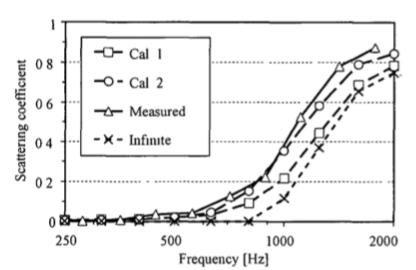
\includegraphics[width=0.7\linewidth]{images/2_diffuse_reflection_rate.png} 
  \caption{ Random incident diffusion coefficient of one-dimensional sinusoidal wall[Messured], Calculated value: Directed correlation method [Cal 1], Sample rotation method [Cal 2], Infinite wall[Infinite](Source: {\it Sakuma et al.}\cite{sakuma2004soundreflection} Fig.9)}
  \label{fig:diffuse_rate}
\end{figure}

\subsubsection{鏡面反射での反射音の振る舞い\label{spec}}
鏡面反射における観測点でのエネルギー$e_\mathrm{spe}$について考える。
式の定義には,光学におけるPhongのモデル\cite{phong1975specularreflection}を参考にした。
Phongのモデルは経験に基づく古典的なモデルであり,次式のように照明方向の正反
射方向と観測方向のなす角$\beta_\mathrm{spe}$の余弦のべき乗として近似するモデルである.
このとき、反射波の強さ$i$は
\begin{equation}
	\label{equ:phong}
	i = \rho_\mathrm{spe}\cos^{n}(\beta_\mathrm{spe}) ,
\end{equation}
と表せる。

このとき、$\rho_\mathrm{spe}$は鏡面反射率であり,鏡面反射の強さを表す.係数$n$は,表面の粗さを表すパ ラメータである。このモデルは,あくまで経験に基づくものであり,エネルギー保存の法則を満たす保証がないなどの性質は気をつける必要はあるが,簡単に計算できるため,今回は使用した。

以上のPhongのモデルを参考にして、鏡面反射音$e_\mathrm{spe}$のエネルギーを式(\ref{equ:e_spe})のように定義した。
\begin{equation}
    \label{equ:e_spe}
      e_\mathrm{spe}(\mathbf{S}, \mathbf{N}, \mathbf{V}, n) = \cos^{n}\beta(\mathbf{S}, \mathbf{N}, \mathbf{V}).
\end{equation}

このとき、$\beta(\mathbf{S}, \mathbf{N}, \mathbf{V})$について反射の法則と余弦定理を用いることで、求めていく。
まず、$\mathbf{S'}$は反射の法則より$\mathbf{S}, \mathbf{N}$を用いて以下のように表すことができる。
\begin{equation}
	\mathbf{S'} = \mathbf{S} + 2(- \mathbf{S}^{\mathrm{T}} \mathbf{N}) \mathbf{N}.
\end{equation}

次に、$\mathbf{V}$と$\mathbf{S'}$のなす角$\beta$は余弦定理より以下の用に表す事ができる
\begin{equation}
	\cos\beta = \frac{\mathbf{S'}^{T}\mathbf{V}}{|\mathbf{S'}||\mathbf{V}|}.
\end{equation}

これより、
\begin{equation}
	\cos\beta(\mathbf{S}, \mathbf{N}, \mathbf{V}) = \frac{(\mathbf{S} + 2(- \mathbf{S}^{\mathrm{T}} \mathbf{N}) \mathbf{N})^{T}\mathbf{V}}{|\mathbf{S} + 2(- \mathbf{S}^{\mathrm{T}} \mathbf{N}) \mathbf{N}||\mathbf{V}|},
\end{equation}

となる。

\subsubsection{拡散反射での反射音の振る舞い\label{diff}}
拡散反射における観測点でのエネルギー$e_\mathrm{dif}$について考える。
拡散反射が入射光が表面層内部で乱反射することで生じる成分であり,観測方向に依存せず,あらゆる方向に均一の強度で観測される.
この式の定義には光学におけるLambertのモデル\cite{micheal1994diffusereflection}を参考にした。
Lambertのモデルは、式(\ref{equ:lambert})のように照明方向と法線方向のなす角の余弦に比例すると仮定する。反射波の強さ$i$は
\begin{equation}
	\label{equ:lambert}
	i = \rho_\mathrm{dif}\mathbf{S}^{\mathrm{T}}\mathbf{N},
\end{equation}
となる。

拡散反射音のエネルギーを式(\ref{equ:e_dif})のように定義した。
\begin{equation}
    \label{equ:e_dif}
    e_\mathrm{dif} = \kappa\mathbf{S}^{\mathrm{T}}\mathbf{N}.
\end{equation}
    
このとき、$\kappa$は拡散反射の中でもマイクに入ってくる音の割合を示す
% 拡散反射における表面の粗さに関係なく一様に拡散反射すると仮定して、鏡面反射のような表面の粗さに関するパラメータは必要ない。

\subsubsection{推定モデルの考察}
平面上のある点Qにおける式(\ref{equ:all-reflection})に式(\ref{equ:gamma}), 式(\ref{equ:e_spe}), 式(\ref{equ:e_dif})を当てはめる。
音源方向$\mathbf{S}$とマイク方向$\mathbf{V}$は既知であるため、この式は音の周波数の高さ$f$と面の方位角方向$\mathbf{N}$の2つが変数となる。
音源方向$\mathbf{S}$とマイク方向$\mathbf{V}$を固定した場合にこの2つの変数において、変化させてみたものを\figref{e_f&N}に示す。
ただし、$\mathbf{V}=(0,-1)$, $\mathbf{S}=(0,-1)$とおいた。そのため、今回の平面とマイク、スピーカの配置では$\mathbf{N} = (-\cos{\psi}, -\sin{\psi})$とした時、$\psi =0$[deg]で最大のエネルギーになる

\begin{figure}[t]
  \centering
  \subfigure[Frequency response of energy $E$($f$) with constant azimuthal direction $\mathbf{N}$ at a point $Q$ on the plane surface]{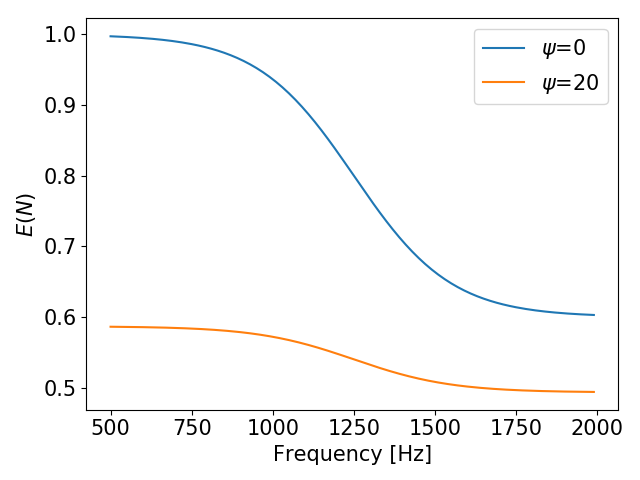
\includegraphics[width=65mm]{images/Re2_e_f.png}\label{fig:e-f}}
  \centering
  \subfigure[Relation between energy $E$($\mathbf{N}$) and azimuth $\mathbf{N}$ when sound frequency $f$ is constant at a certain point $Q$ on the plane surface]{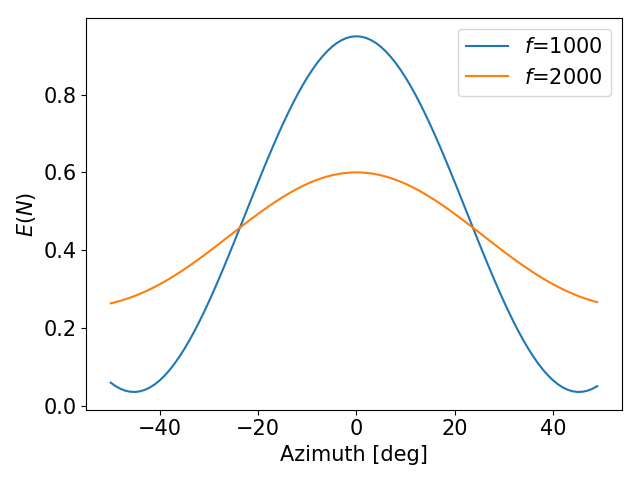
\includegraphics[width=65mm]{images/Re2_e_N.png}\label{fig:e-n}}
 \caption{Relationship between energy (E) change with respect to frequency (f) and azimuth direction (N) when the sound source direction (S) and microphone direction (V) are fixed in the model}\label{fig:e_f&N}
\end{figure}

\figref{e-f}のように、横軸を周波数でとると、エネルギーの周波数応答を見ることができる。よって、鏡面反射成分と拡散反射成分では鏡面反射のほうが強いため前半のほうが大きく、周波数が高くなるにつれて小さくなっていることがわかる。方位角の例として、$\psi=0, \psi=20$の時を比べてみると、確かに$\psi=0$のほうが大きくなっている

つぎにに\figref{e-n}のように、横軸を方位角を取ると、エネルギーと角度の関係がわかりやすい。また、周波数で比べてみても鏡面反射成分が強い$f=1000$のほうが大きく変化していることがわかる。

最後に、物体面の方位角と中域($f_m$[Hz])、高域($f_h$[Hz])での比$D$との関係について考えると, $D$は$\mathbf{N}$のみが変数となり、以下のような式(\ref{eq:d_n_fm_fh})になる
\begin{equation}
	\label{eq:d_n_fm_fh}
	D(\mathbf{N}) = \frac{E(\mathbf{N}|f_{m})}{E(\mathbf{N}|f_{h})}.
\end{equation}

また、これを図に表してみると、\figref{d-n}の用になる。

$-50< \psi < 50$の範囲で方位角に対して、エネルギーの比$D$が関係するモデルを作成することができた。このとき、音源の入射方向$\mathbf{S} = (-\cos{_\phi}, -\sin{_\phi})$ (0[deg] < $_\phi$ < 180[deg])とする。
$D$と$N$の関係の図より、物体の方位角を式(\ref{eq:d_n_fm_fh})から求める場合、二通りの解き方が考えられる。一つは方位角を制限する。$_\phi=90$[deg]の場合$0<\psi<50$の範囲に制限することで、単調減少するため一意に求める事ができる。
もう一つは複数方向からの音源を用意することである。\figref{d-n}でもあるように$_\phi=90$[deg]だけでは一意には求めることができないが、複数方向からの音源例えば、$_\phi = 45$[deg]があれば、連立方程式より求めることが可能になる。

これより、この$D$を$\mathbf{N}$に関して方程式を解く事によって、方位角方向$\mathbf{N}$を推定することができる。

\begin{figure}[t]
  \begin{center}
  \vspace{1zh}
    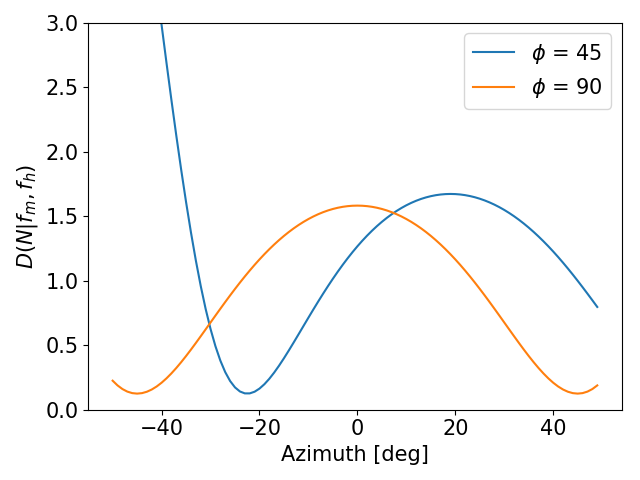
\includegraphics[width=0.7\linewidth]{images/Re2_d_n.png}   
  \end{center}
  \caption{Relation between energy ratio $D(\mathbf{N}|f_m, f_h)$ and azimuth angle $\mathbf{N}$ between mid and high frequencies at a point Q on the plane($f_m = 1000$, $f_h = 2000$)}
  \label{fig:d-n}
\end{figure}

\subsection{SVRを用いた方位角推定}
\label{sec:svr_method}

\subsubsection{データセット作成方法}
\label{sec:make_data_set}
音のデータを作成するフローについて、\figref{flow_data_set}に示す。フローについて、順番に示す。

まず、実験データから使用する音を切り取る。このとき、ゼロクロス検出を用いる。ゼロクロス検出とは、ある区間において正から負、もしくは負から正に値が移動した回数を数えることで信号の周波数等変化を認識が可能である。これにより、周波数の変化をフーリエ変換なしに見ることができる。今回使用している音波は徐々に周波数が大きくなる音を使用しているため、最初の音の起こりは認識しづらいが音の終わりはわかりやすいため、今回使用した音のゼロクロスの結果と周波数の結果の比較の図を\figref{compare_stft_0cross}に示す。

このように、ゼロクロスの値が音が終わるさいに急激に落ちる。このときの値を音が終わる時間として、それ以前の約1 [秒]のデータを今回の実験データとして使用する。

次に周波数領域になおす。音のデータセットを作成する際には時間領域のデータでは、雑音の影響を受ける。そのため、フーリエ変換を用いる。このときのフーリエ変化では、高速フーリエ変換を用いる。このとき、フーリエ変換のパラメータとして、窓関数は周波数分解能が良いハミング窓、サンプリング周波数は44100 [Hz]、データ数は45120 [個](データ時間は約1 [秒])を用いた。

最後にデータを整理する。今回は\secref{self_by_myself}でも示したが、1000 [Hz]から2000 [Hz]の変化に着目するため、まず、1000 [Hz]から2000[Hz]のデータのみで切り取る。次に、変化を見るために、平均0分散1で正規化を行う。最後に、ノイズを減らすために平滑化を行う。今回は周波数領域において、移動平均法を用いた。このとき、平滑化の幅は512 [個]のデータごとで行っている。

\begin{figure}[ht]
  \begin{center}
  \vspace{1zh}
    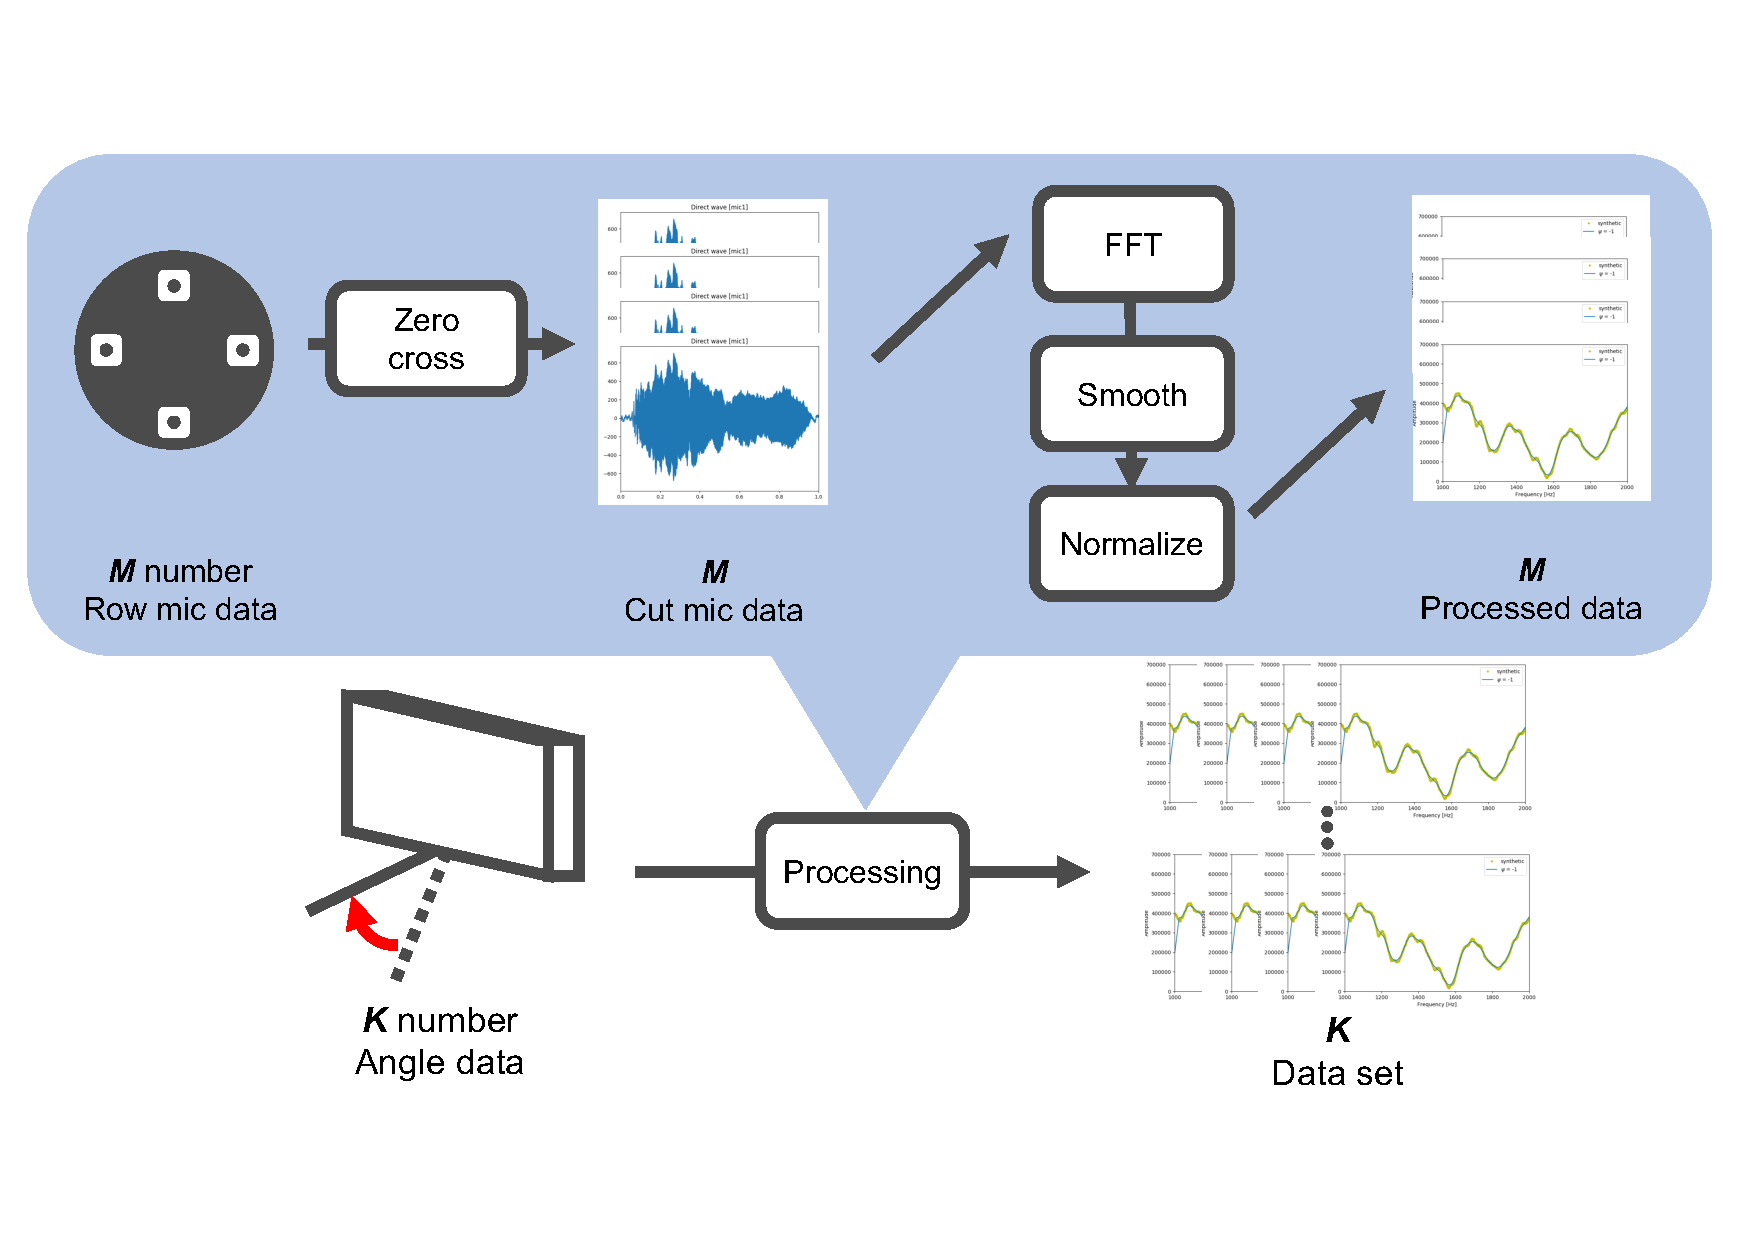
\includegraphics[width=\linewidth]{images/2_how_to_make_data_set.pdf}   
  \end{center}
  \vspace{-2zh}
  \caption{Flowchart to create dataset}
  \label{fig:flow_data_set}
\end{figure}

\begin{figure}[ht]
  \centering
  \subfigure[Zero cross]{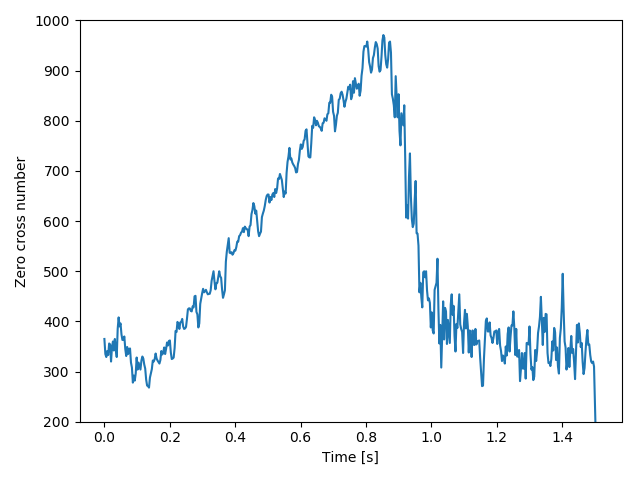
\includegraphics[width=0.45\linewidth]{images/2_zerocross.png}}
  \label{fig:0cross}
  \centering
  \subfigure[Short-time fourier transform]{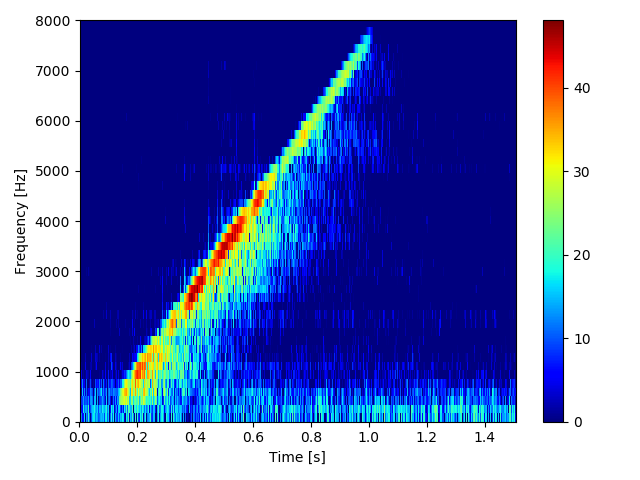
\includegraphics[width=0.45\linewidth]{images/2_stft.png}}
  \label{fig:stft}
 \caption{Comparison between Zero cross and Short-time fourier transform}\label{fig:compare_stft_0cross}
\end{figure}

\subsubsection{サポートベクター回帰}
\label{sec:support_vector_regression}
本研究では、平面の方位角を推定するのに、サポートベクター回帰(Support Vector Regression: 以降 SVR)を用いる。\cite{bishop2011prml}SVRの特徴として、誤差に不感帯を設けることで、ノイズの影響を受けにくく、さらに、基本的には線形な回帰分析手法であるが、カネールトリックを使うことによって、非線形の回帰モデルになる。本研究では、ガウシアンカーネルの非線形の回帰モデルを用いることで、対象平面の方位角推定を行う。

以下にSVRの簡単な理論について説明する。

非線形SVRでは、次を最小化する係数を求めます。

\begin{equation}
    L(\alpha) = \frac{1}{2}\sum^{N}_{i=1}\sum^{N}_{j=1}(\alpha_i - \alpha^{\ast}_i)(\alpha_j - \alpha^{\ast}_j)G(x_i, x_j) + \epsilon\sum^{N}_{i+1}(\alpha _i + \alpha^{\ast}_i) - \sum^{N}_{i=1}y_i(\alpha_i-\alpha^{\ast}_i)
\end{equation}

これには、次の条件が適用される。
\begin{equation}
    \begin{array}{l}
        \sum^{N}_{n=1} (\alpha_n - \alpha^{\ast}_n) = 0\\
        \forall n : 0 \le \alpha_n \le C\\
        \forall n : 0 \le \alpha^{\ast}_n \le C.
    \end{array}
\end{equation}

条件より、推定に使用される関数は以下に等しくなる。

\begin{equation}
    f(x) = \sum^{n}_{i=1}(\alpha_i - \alpha^{\ast}_i)G(x{n},x) + b
\end{equation}

このとき、Gは非線形カーネル関数で以下のように考えられる。

\begin{equation}
    G(x_n, x) = \mathrm{exp}(-\gamma||x_n=x||^{2})
\end{equation}

$\alpha_n, \alpha^{\ast}_n$が誤差$\epsilon$の範囲内にない場合に$\alpha_n - \alpha^{\ast}_n = 0$となり、SVRの回帰式を作成するサンプルとなる。$\epsilon = 0$のときが最もノイズに強いモデルとなる。。

このとき, C, $\gamma$, $\epsilon$の3つがハイパーパラメータとして存在する。しかし、Cは$\epsilon$から導くこともできるため、C, $\gamma$の二つのパラメータを求める。この2つのハイパーパラメータを求めるためにグリッドサーチ交差検証を行う。グリッドサーチ交差検証とは、モデルの精度を向上させるために用いられる手法であり、全てのパラメータの組み合わせを試すグリッドサーチに加えて、さらにテストデータと訓練データの組み合わせを試す交差検証をすることで、最も評価精度が高いパラメータを探索する手法である。
今回、この評価指標として、決定係数($\mathrm{R}^2$ Score)を採用した。

\clearpage
\newpage